\section{Introduction}

The reproducibility crisis identified in machine learning \citep{kapoor2022leakage} highlights the critical necessity for replication and validation in research. 
Our investigation focuses on reproducing and extending the work by \citealp{ling2023learning}, which proposed a fair learning method for Graph Neural Networks (GNNs; \citealp{kipf2017semisupervised}).

GNNs have shown considerable performance \citep{gao2019graph, liu2021fast, liu2021dig, yuan2021explainability} across multiple domains \citep{hamaguchi2017knowledge, liu2022spherical, han2022g, hamilton2017inductive}. 
Despite this success, GNNs have been shown to carry over or amplify bias present in training data \citep{dai2021say, mehrabi2021survey, olteanu2019social}. Specifically, the output of neural networks can be substantially correlated with sensitive features such as ethnicity, nationality, and gender, even though this behavior might not have been intended  \citep{dai2021say}.
Such biases can be present in graph data, hidden in both the way nodes are connected and their features \citep{mehrabi2021survey, olteanu2019social}. 
Moreover, removing sensitive features does not always lead to a fairer dataset, as the sensitive information can be retrieved from other features or their combinations \citep{sweeney2002k}.

To tackle this issue, previous approaches for fair graph models have employed various pre-processing techniques (i.e. augmenting the data to remove bias before training the actual network).
Some augmentation-based methods used handcrafted heuristics for changing the training data \citep{spinelli2021fairdrop, kose2022fair}. Building upon this foundation, \citet{ling2023learning} propose \textit{Graphair}, a framework focused on learning data augmentations that remove bias from a dataset. 
The authors claim that this method considerably improves on common group fairness metrics across multiple datasets compared to other fair graph training schemes while achieving similar performance in terms of accuracy. We reproduce the experiments by \citet{ling2023learning} to verify their main claims, as well as extend the tests of the method to examine its generalizability and robustness. More specifically, our contributions are summarized below:
\begin{enumerate}
    \item We repeat all experiments from the original paper by \citet{ling2023learning}.

    \item We alter the evaluation procedure to retrain the entire method five times with different random seeds, thereby achieving a more robust assessment of the method's stability and performance.
    
    \item We assess how well the method generalizes to different architectures.
    
    \item We conduct further ablation studies to investigate how the individual components of the Graphair framework contribute to improving fairness.
    
    \item We run additional experiments with synthetic datasets to assess the stability and performance of Graphair for datasets with different homophily. 
    
    \item We improve the readability and reproducibility of the given code.
\end{enumerate}

\section{Scope of Reproducibility}

\citet{ling2023learning} propose a technique that automatically learns augmentations that change both the adjacency matrix and the node embeddings of a graph by incorporating adversarial and contrastive learning approaches. We identify the following claims from the paper:
\begin{itemize}[leftmargin=*]
    \item[]\textbf{Claim 1:}\claim{claim:1} Learned augmentations \textbf{improve group fairness metrics} while retaining \textbf{similar accuracy} compared to other fair graph-learning methods, on datasets containing sensitive attributes.
    \item[]\textbf{Claim 2:}\claim{claim:3} \textbf{Augmenting both edges and node features} achieves \text{higher accuracy and better fairness} scores than just augmenting one of them.
    \item[]\textbf{Claim 3:}\claim{claim:4} Learned augmentations \textbf{reduce node-wise sensitive homophily and correlation} between node features and the sensitive attribute.
\end{itemize}

\section{Methodology}
 We use the code provided by the authors\footnote{\url{https://github.com/divelab/DIG}}, with various improvements, such as setting random seeds for reproducibility, putting all the hyperparameters into a single file to make further replication and experimentation easier, adding missing functionality that was described in the paper, but did not appear in the codebase, as well as bug fixes. 
 It is important to mention that the code provided by the authors is not the original code they used for running the experiments. Therefore, we attempt to make the code as similar to the settings described in the paper as possible. 
 We also extend the authors' work with further experiments, which we describe in section \ref{experimental-setup}. The code for the reproduction and extensions is available online\footnote{\url{https://github.com/Thiggel/FACT}}.


\subsection{Graphair framework overview}
Given a graph $G = \{A, X, S\}$ with an adjacency matrix $A$, node features $X$, and the sensitive feature $S$, the Graphair method employs an augmentation module $g$ to produce fair augmented data, an adversary $k$ to ensure fairness, and a GNN-based encoder $f$ to produce node-embeddings for downstream tasks. The three components are described in detail below.


\subsubsection{Augmentation Module}

The augmentation module $g$ first uses a Graph Convolutional Network (GCN; \citealp{kipf2017semisupervised}) encoder $g_{enc}$ to obtain node embeddings $Z = g_{enc}(A, X)$. 
The embedding $Z$ is used to create a new graph $G' = \{A', X', S\}$
$$
Z_A = \operatorname{MLP}_A(Z), \quad \widetilde{A^{\prime}} = \sigma\left(Z_A Z_A^T\right),
\quad A_{i j}^{\prime} \sim \operatorname{Bernoulli}\left(\widetilde{A^{\prime}}{ }_{i j}\right) \text { for } i, j=1, \cdots, n
$$
$$
Z_X = \operatorname{MLP}_X(Z), \quad
\widetilde{M} = \sigma\left(Z_X\right), \quad
M_{i j} \sim \operatorname{Bernoulli}\left(\widetilde{M}_{i j}\right) \text { for } i, j=1, \cdots, n
$$
$$X^{\prime}=M \odot X
$$

where $\operatorname{MLP}_A$ and $\operatorname{MLP}_X$ are two Multi-Layer Perceptrons (MLPs), $\sigma$ is the sigmoid function, and $\odot$ is the Hadamard product.
$\operatorname{MLP}_A$ and $\operatorname{MLP}_X$ both have two linear layers, separated by a ReLU activation function.
To make the sampling process differentiable, the Gumble-Softmax reparameterization trick is employed \citep{jang-reparameterization}.


\subsubsection{Adversarial Training}

To ensure fairness, Graphair uses adversarial training: a GCN with an MLP head is defined as the adversary $k: (A', X') \xrightarrow{} \hat{S} \in [0, 1]^n$, which predicts the sensitive attribute $S$ from the augmented adjacency matrix $A'$ and masked node embeddings $X'$.
The adversarial module $k$ is trained together with the augmentation module $g$ in an adversarial fashion, utilizing an adversarial loss $L_{\mathrm{adv}}$. 
While the adversarial module tries to predict the sensitive feature from $A'$ and $X'$, the augmentation module is trained so that $A'$ and $X'$ do not contain bias, making it difficult for the adversary to recover the sensitive attribute.
The adversarial training procedure can formally be described as the following optimization problem:

$$\min _g \max _k L_{\mathrm{adv}} = \min _g \max _k -L_{\text{BCE}}\left(S_i, \hat{S}_i\right)$$

where $L_{\text{BCE}}$ denotes binary cross-entropy, $S_i$ denotes the sensitive feature and $\hat{S}_i$ denotes the prediction of the sensitive feature by the adversary.

\subsubsection{Contrastive Learning and Reconstruction Loss}

Additionally, to avoid the loss of information and converging to a trivial solution, a contrastive learning objective $L_{\mathrm{con}}$ is used, which maximizes agreement between the representations of the original graph and the augmented one. These representations are denoted $h$ and $h'$ respectively and are learned by the GNN-based encoder $f$:
$$
L_{\mathrm{con}}=\frac{1}{2 n} \sum_{i=1}^n\left[l\left(h_i, h_i^{\prime}\right)+l\left(h_i^{\prime}, h_i\right)\right]
$$
where $l\left(a, b\right)$ denotes the contrastive learning objective defined by \citet{zhu2020deep}.


Finally, a reconstruction loss term $L_{\text {rec }}$ is added to avoid large deviations of the augmented graph from the original graph.

$$
L_{\text{rec}} = L_{\text{BCE}}\left(A, \widetilde{A^{\prime}}\right)+\lambda L_{\text{MSE}}\left(X, X^{\prime}\right)
$$ where $L_{\text{BCE}}$ and $L_{\text{MSE}}$ denote binary cross entropy and mean squared error, $\widetilde{A^{\prime}}$ refers to the edge probability matrix obtained from the augmentation module, and $\lambda$ is a hyperparameter.

The overall training process can be described by the following min-max optimization problem:

$$
\min_{f, g} \max_k L = \min_{f, g} \max_k \alpha L_{\text{adv}} + \beta L_{\text{con}} + \gamma L_{\text{rec}}
$$

where $\alpha$, $\beta$ and $\gamma$ are hyperparameters. This scheme defines a self-supervised training regime that aims to produce a fair GNN-based encoder $f$ as the end product for being used in downstream tasks. Appendix \ref{fig:original-framework} shows a visual overview of the framework.

\subsection{Evaluation}\label{Evaluation_protocol}
To evaluate the Graphair framework, the embeddings produced by the trained encoder are used for a downstream task. For this purpose, a simple MLP classifier is trained on the embeddings to predict a binary target attribute $Y$.
The classifier's performance is measured by its test accuracy, as well as two group fairness metrics: Demographic Parity $\Delta\text{DP}$ and Equal Opportunity $\Delta\text{EO}$ \citep{louizos2015variational, beutel2017data}, which are defined as follows:
$$\Delta\text{DP} = |P(\hat{Y}=1|S=0) - P(\hat{Y}=1|S=1)|$$ 
$$\Delta\text{EO} = |P(\hat{Y}=1|S=0, Y=1) - P(\hat{Y}=1|S=1, Y=1)|$$ 
where $\hat{Y}$ is the prediction of the classifier, $Y$ is the true target label, and $S$ is the sensitive feature. The MLP network consists of 2 linear layers with a ReLU activation in between. The classifier is trained 5 times and the average metrics are reported.

\subsection{Datasets}\label{sec:datasets}

For the replication, we use the same three datasets as the original paper: NBA, Pokec-z, and Pokec-n
\citep{DBLP:journals/corr/abs-2009-01454}. 
We further create new synthetic datasets to verify the generalizability of the claims made by the authors. 

\subsubsection{Original Paper Datasets}

\textbf{NBA}: Nodes represent basketball players. Features include nationality, age, salary, and several performance statistics.
The edges are based on whether players follow each other on social media. 
The sensitive feature is nationality, and the classification task is to predict whether a player's salary is above the median.

\textbf{Pokec}: The data comes from a popular social network in Slovakia, and is separated into two subsets by region: Pokec-z and Pokec-n. The nodes in the graph are the users, and the features are information about the users. The region of the users is treated as the sensitive feature. The classification task is to predict the working field of the users.


\subsubsection{Additional Datasets}

To test the claim that Graphair works well regardless of graph structure and connectivity, we create a synthetic dataset (in five variants, to be explained below) using the DPAH module \citep{espin2022inequality}, composed of people as nodes and their friendships as edges. The dataset has a majority group and a minority group, the latter of which might, for example, correspond to a racial minority. Each node has three attributes: 
\begin{itemize}
    \item Group membership (binary, \textit{majority} or \textit{minority}) – 70\% of the nodes are majority while 30\% are minority.
    \item Education (binary, \textit{good} or \textit{bad}) – 70\% of majority nodes have good education, while only 30\% of minority nodes have good education.
    \item Income (binary, \textit{high} or \textit{low}) – 90\% of majority nodes have high income, while only 10\% of minority nodes have high income.
\end{itemize}

Hence, education correlates with group membership, while group membership in turn correlates with income.

The task for a GNN classifier is to predict the income based on group membership and education.
Graphair aims at not only deleting the sensitive attribute (which would be trivial) but also completely decorrelating it from other attributes, as it is possible to recover sensitive attributes from other attributes \citep{sweeney2002k}. 
In this case, the education attribute can be used to predict the group membership with high accuracy, as the two correlate. From there on, the classifier would be able to deduce income. 
Therefore, it would be detrimental if Graphair only deleted the attribute ``group membership'', as the classifier could still easily learn to represent group membership as a latent variable and deduce income from it. 
In other words, if Graphair were able to fully decorrelate the sensitive feature from other features, it would need to fully mask both the education and the group membership attribute. 
That way, the classifier would only get nonsense information and have no other optimal choice than always output “high income” no matter the input, for which the accuracy would go to 66\% (the percentage of high-income nodes in the dataset, i.e., the prior probability of having high income). 
Simultaneously, the classifier would achieve perfect fairness in this case. While in normal scenarios, masking the entire dataset input would not be useful, we create this isolated setting in which we can clearly assess the claims of Graphair as all dataset features correlate with the sensitive attribute.

Having created this isolated test setting, we now vary graph connectivity. We want to test the generalizability of Graphair to differently connected graph datasets, as in real-world settings, e.g., minority groups may be segregated in different ways.
Specifically, if nodes connect often within their group but scarcely between groups, or vice-versa, Graphair should still work fine. 
This tendency to connect within or amongst groups is known as homophily \citep{espin2022inequality}. 
The way nodes connect determines the information flow within the GNN and thus influences the prediction of a GNN classifier.
We test whether (1) Graphair is capable of decorrelating the features at all in this setting and (2) whether this decorrelation breaks for certain graph connectivities (homophilies).
We use a range of different graph connectivity configurations, creating five variations of the synthetic dataset:

\begin{enumerate}
    \item Low connectivity both inside minority and majority group (called Syn-0.2-0.2). In this case, most friendships are between minority and majority people.
    \item Low connectivity inside minority group and high connectivity inside majority group (called Syn-0.2-0.8).
    \item Medium connectivity both inside minority and majority nodes (called Syn-0.5-0.5). This implies medium connectivity between minority and majority nodes as well.
    \item High connectivity inside minority group and low connectivity inside majority group (called Syn-0.8-0.2).
    \item High connectivity both inside minority and majority group (called Syn-0.8-0.8). In this case, few friendships exist between minority and majority people.
\end{enumerate}

E.g., for Syn-0.2-0.8, the first value (0.2) refers to the tendency of minority nodes to connect to each other (i.e., homophily), while the second one (0.8) denotes the tendency of majority nodes to connect to each other. Simultaneously, minority nodes connect to majority ones often in this case, while majority nodes seldom connect to minority nodes. Thus, in this particular example, there are few friendships between minority and minority persons, and many between majority and majority persons. For further information on homophily, we refer to appendix \ref{appendix:homophily}.


Table \ref{tab:datasets} shows all relevant dataset statistics, as well as the specific homophily settings used for the synthetic dataset creation.

\begin{table}[t]
    \centering
    \caption{Dataset statistics. Synthetic datasets are made up of 700 majority and 300 minority nodes. The first number in the synthetic dataset names refers to the homophily of minority nodes (also shown in the second last column) while the second number refers to the homophily of majority nodes (also shown in the last column).}
    \begin{tabular}{lccccccc}
        \textbf{Dataset} & \textbf{Nodes} & \makecell{\textbf{Node}\\\textbf{features}} & \textbf{Edges} & \makecell{\textbf{Inter-group}\\\textbf{edges}} & \makecell{\textbf{Intra-group}\\\textbf{edges}} & 
        \makecell{\textbf{min.}\\\textbf{Hom.}} & \makecell{\textbf{maj.}\\\textbf{Hom.}} \\
        \midrule\\
        \textbf{NBA} & 403 & 39 & 16,570 & 4,401 & 12,169 & \multirow{3}*{-} & \multirow{3}*{-} \\
        \textbf{Pokec-z} & 67,797 & 59 & 882,765 & 39,804 & 842,961 & & \\
        \textbf{Pokec-n} & 66,569 & 59 & 729,129 & 31,515 & 697,614 & & \\\\
        \hline\\
        \textbf{Syn-0.2-0.2} & \multirow{5}*{1,000} & \multirow{5}*{3} & \multirow{5}*{29,970} & 23,695 & 6,275 & 0.2 & 0.2 \\
        \textbf{Syn-0.2-0.8} & &  &  & 20,470 & 9,500 & 0.2 & 0.8 \\
        \textbf{Syn-0.5-0.5} & &  &  & 12,557 & 17,413 & 0.5 & 0.5 \\
        \textbf{Syn-0.8-0.2} & &  &  & 9,107 & 20,863 & 0.8 & 0.2 \\
        \textbf{Syn-0.8-0.8} & &  &  & 5,841 & 24,129 & 0.8 & 0.8 \\
    \end{tabular}
    \label{tab:datasets}
\end{table}

\subsection{Experimental setup}\label{experimental-setup}

\subsubsection{Original Experiment}
\label{sec:original-experiment}

\textbf{Claim \ref{claim:1}}: Following the methodology of the authors, we conduct a grid search over the values 0.1, 1, and 10 to find the hyperparameter setting for $\alpha$, $\gamma$, and $\lambda$ that results in the best model in terms of average accuracy over 5 evaluation runs. 
The experiment is repeated for all three datasets: NBA, Pokec-z, and Pokec-n. Due to the size of Pokec datasets being significantly larger than others, batch training is used, where, following the method described in \citep{Zeng2020GraphSAINT}, one batch is created using random walk sampling with 1000 root nodes and walk length 3. This procedure results in batches of at most 3000 nodes.

\textbf{Claim \ref{claim:3}}: The verification of this claim is addressed in an ablation study: we run our evaluation protocol while disabling the respective components of the augmentation module individually. Appendix \ref{fig:ablation} shows a graphic of this alteration.

\textbf{Claim \ref{claim:4}}: To address this claim, we investigate how node-wise sensitive homophily (i.e., the tendency of nodes to connect with nodes having the same sensitive attribute value) and Spearman correlation between the sensitive and other features decrease in the fair setting.

\subsubsection{Change of Experimental Setup for Better Robustness Assessment}

As described in Section \ref{Evaluation_protocol}, to evaluate the Graphair framework the authors train the models $f$, $k$, and $g$ once in an unsupervised manner, and then train a classifier 5 times to obtain the mean and variance of the results. 
However, this procedure does not show how robust and stable the actual proposed method (Graphair) is, but only how much variation in results the simple classifier undergoes throughout different runs. 
A more appropriate approach would be to test the stability of Graphair itself. 
Therefore, we conduct a second experiment, where models $f$, $k$, and $g$ are trained five times, together with the classifier.
All further experiments use this approach. Diagrams of the two evaluation protocols are shown in appendix \ref{appendix:evaluation-protocols}.

\subsubsection{Longer Training Procedure}
In the original paper, the authors claim that Graphair is trained on Pokec datasets for 500 epochs. 
However, upon reviewing the codebase, we discovered that the code did not implement mini-batch training correctly,  resulting in the term ``epochs'' being used inaccurately to refer to steps.\footnote{We contacted the authors about this bug. Since then, it has been fixed by the authors.} 
We contacted the authors to obtain the appropriate parameters for running the code, and they supplied parameters corresponding to 500 steps of training.

Given that the full dataset contains approximately 66,000 nodes and mini-batches of up to 3000 nodes are used, it would require 22 steps to cover the entire dataset once. 
Therefore, to train the model for 500 epochs, the total number of steps should be equal to 11,000 ($=500\cdot22$).

To thoroughly evaluate Graphair, we train the model for both 500 and 11,000 steps. 
Due to computational limitations, we conduct a grid search as detailed in Section \ref{sec:original-experiment} using 500 steps and subsequently re-run the experiments with the optimal hyperparameters for 11,000 steps. 
Unless specified otherwise, all further experiments use the models obtained from this longer training procedure.


\subsubsection{Further Experiments to Verify Claims}\label{further_experiments}

To further test whether the proposed method improves fairness in comparison to unfair methods (\textbf{Claim \ref{claim:1}}), we carry out two additional experiments.

\textbf{Examining the effects of adversarial training}:
To validate the effect of adversarial training on the performance of the model, we train Graphair with hyperparameter $\alpha=0$, which corresponds to not using the adversarial loss. 
Under such a setting, we expect fairness to deteriorate, and accuracy to improve (compared to training with a nonzero value like $\alpha=1$) because the augmentation module no longer makes use of adversarial training to satisfy the fairness property. Appendix \ref{fig:without-adversarial} shows a visual overview of this alteration.

\textbf{Comparison to unfair baseline}:
Graphair consists of two parts: a fairness step which produces a fair graph, and a finetuning step which trains a classifier on that graph. 
The novelty of Graphair lies in the first step, while the second step is a standard downstream performance evaluation procedure. 
Even though the authors claim that their method results in much fairer graphs compared to the other graph fairness frameworks, they never compare their method against the "unfair" baseline.

To assess the actual benefits of employing Graphair, compared to not doing any fairness training, we turn off the fairness step and train the classifier on the original graph directly. 
This serves as a sanity check for the method, as we expect Graphair's fairness step to lead to improved fairness as compared to the unfair baseline. 
Appendix \ref{fig:supervised} shows a visual overview of this alteration. 

\subsubsection{Additional Experiments to Verify Graphair’s Generalizability}

To test the generalizability of the proposed method, we conduct the following experiments:

\textbf{Generalizability to different GNN architectures}: To investigate whether the method generalizes beyond GCNs to other Message-Passing GNNs \citep{gilmer2017neural}, we modify the experimental setup, replacing all GCNs with Graph Attention Networks (GATs; \citealp{velivckovic2017graph}). This verifies \textbf{Claim \ref{claim:1}} in regards to whether the high accuracy and good fairness results hold in this case. Similarly to \ref{sec:original-experiment} we perform a full grid search to find the best hyperparameters.

\textbf{Generalizability to graphs with varying homophily}: We examine whether the method generalizes to different graph structures. To that end, we repeat the experiment on all five synthetic datasets described in Section \ref{sec:datasets}.

\subsection{Computational Requirements}

We used a single NVIDIA RTX A6000 GPU for running the experiments. 
On this GPU, the average Graphair runtime per hyperparameter setting is around 3 minutes for models trained on Pokec datasets for 500 steps, 30 minutes for models trained for 11,000 steps, and around 30 seconds for models trained on the NBA dataset. 
In total, we trained 650 models.
All experiments combined took a total of 119 GPU hours.

\section{Results}

\subsection{Results Verifying Original Claims}

\begin{table}[t]
    \caption{The results on the NBA, Pokec-z, and Pokec-n datasets, showing the original and the reproduced results with an identical experimental setup, the results employing our proposed evaluation protocol, and the longer training results.}
    
    \label{tab:reproduction}
    \centering
    \begin{tabular}{lllccc}
        \bf DATASET & \multicolumn{1}{c}{\bf SETTING} & \makecell{\bf EVALUATION\\\bf PROTOCOL} & \bf ACCURACY $\uparrow$ & $\Delta$ \bf DP $\downarrow$ & $\Delta$ \bf EO $\downarrow$ \\
        \hline\\
        \multirow{3}*{NBA} & original & original & $69.36 \pm 0.45$ & $2.56 \pm 0.41$ & $4.64 \pm 0.17$\\
        & reproduction & original & $\mathbf{69.64} \pm \mathbf{0.69}$ & $\mathbf{0.14} \pm \mathbf{0.00}$ & $3.98 \pm 0.87$\\
        & reproduction & ours & $69.36 \pm 0.46$ & $2.57 \pm 1.13$ & $\mathbf{2.33} \pm \mathbf{1.53}$\\\\
        \hline\\
        \multirow{3}*{Pokec-z} & original & original & $\mathbf{68.17} \pm \mathbf{0.08}$ & $2.10 \pm 0.17$ & $2.76 \pm 0.19$\\
        & reproduction & original & $61.83 \pm 0.29$ & $\mathbf{1.48} \pm \mathbf{0.79}$ & $3.97 \pm 1.06$\\
        & reproduction & ours & $60.60 \pm 1.97$ & $2.84 \pm 2.04$ & $3.59 \pm 1.96$ \\
        & \makecell[l]{reproduction\\(longer training)} & ours & $63.39 \pm 0.68$  & $2.28 \pm 1.52$  & $\mathbf{2.24} \pm \mathbf{1.99}$ \\\\
        \hline\\
        \multirow{3}*{Pokec-n} & original & original & $\mathbf{67.43} \pm \mathbf{0.25}$ & $\mathbf{2.02} \pm \mathbf{0.40}$ & $\mathbf{1.62} \pm \mathbf{0.47}$ \\
        & reproduction & original & $63.58 \pm 0.30$ & $3.80 \pm 0.43$ & $3.83 \pm 0.60$\\
        & reproduction & ours & $62.64 \pm 0.84$ & $3.82 \pm 2.99$ & $3.98 \pm 2.60$\\
        & \makecell[l]{reproduction\\(longer training)} & ours & $63.88 \pm 0.91$  & $2.85 \pm 0.59$  & $2.40 \pm 1.14$ \\
    \end{tabular}
\end{table}


\begin{table}[t]
    \caption{Setting alpha to zero, compared to its optimal value obtained through the grid search.}
    \label{tab:unfair-alpha}
    \centering
    \begin{tabular}{lcccc}
        \bf DATASET & \multicolumn{1}{c}{\bf $\alpha$} & \bf ACCURACY $\uparrow$ & $\Delta$ \bf DP $\downarrow$ & $\Delta$ \bf EO $\downarrow$ \\
        \hline\\
        \multirow{2}*{NBA} & optimal& $\mathbf{69.36} \pm \mathbf{0.45}$ & $\mathbf{2.57} \pm \mathbf{1.13}$ & $\mathbf{2.33} \pm \mathbf{1.53}$\\
        & 0 & $69.08 \pm 1.71$ & $5.09 \pm 2.30$ & $5.26 \pm 2.54$\\\\
        \hline\\
        \multirow{2}*{Pokec-z} 
        & optimal & $\mathbf{63.39} \pm \mathbf{0.68}$  & $2.28 \pm 1.52$  & $2.24 \pm 1.99$ \\
        & 0 & $62.87 \pm 1.22$ & $\mathbf{1.70} \pm \mathbf{0.6}$ & $\mathbf{2.14} \pm \mathbf{1.64}$\\\\
        \hline\\
        \multirow{2}*{Pokec-n} 
        & optimal & $63.88 \pm 0.91$  & $\mathbf{2.85} \pm \mathbf{0.59}$  & $\mathbf{2.40} \pm \mathbf{1.14}$ \\
        & 0 & $\mathbf{64.57} \pm \mathbf{0.48}$ & $4.72 \pm 1.44$ & $4.34 \pm 1.91$\\
    \end{tabular}
\end{table}

\textbf{Claim \ref{claim:1} (group fairness improvement and similar accuracy)}: In table \ref{tab:reproduction}, we show the results of running a grid search with the original paper's evaluation protocol and our proposed one, as described in section \ref{Evaluation_protocol}. In addition, we report the results of a longer training procedure on both Pokec datasets. 
On the NBA dataset, the results are fully reproduced with both evaluation protocols. 
In some cases, measurements even show a slight improvement in accuracy and fairness metrics. 
The accuracy on the Pokec datasets drops by several percentage points (around $5\%$ for Pokec-z and $4\%$ for Pokec-n), while the fairness is close to the original results. 
It is important to note that the variance in the runs with our evaluation protocol is substantially higher in nearly all cases, especially on the fairness metrics. 
This indicates instability in Graphair's results. 
We present the results achieved using the hyperparameters that lead to optimal fairness. We report primarily these results because, under the settings optimized for the highest accuracy, the fairness was notably worse.
The best accuracy results can be found in appendix \ref{appendix:best-accuracy} and accuracy-fairness trade-off plots can be found in appendix \ref{appendix:pareto-fronts}.

Table \ref{tab:unfair-alpha} shows the results of disabling adversarial training as described in section \ref{further_experiments}. 
For NBA and Pokec-n datasets, we observe higher DP and EO values (at least twice as high compared to the full method), which is expected. 
However, the results on the Pokec-z dataset show that the network without adversarial training leads to similar or even lower values compared to the full model. 
This indicates that the adversarial training does not lead to better graph fairness on this dataset, which again shows Graphair's instability. 
Therefore, this experiment provides only partial evidence for the reproducibility of \textbf{Claim \ref{claim:1}}.

Table \ref{tab:unfair-supervised} shows the results of comparing Graphair to an unfair baseline, which we established by excluding the fairness component from the pipeline.
Compared to Graphair, fairness is worse in the baseline setting on the NBA and Pokec-z datasets, but better on Pokec-n, providing again only partial evidence for \textbf{Claim \ref{claim:1}}. 
Further discussion on these results can be found in section \ref{section:discussion}.

\begin{table}[t]
    \caption{Comparison of Graphair to not using fairness training.}
    \label{tab:unfair-supervised}
    \centering
    \begin{tabular}{llccc}
        \bf DATASET & \multicolumn{1}{c}{\bf SETTING} & \bf ACCURACY $\uparrow$ & $\Delta$ \bf DP $\downarrow$ & $\Delta$ \bf EO $\downarrow$ \\
        \hline\\
        \multirow{2}*{NBA} & full Graphair method & $\mathbf{69.36} \pm \mathbf{0.45}$ & $\mathbf{2.57} \pm \mathbf{1.13}$ & $\mathbf{2.33} \pm \mathbf{1.53}$\\
        & w/o fairness training & $68.65 \pm 2.03$ & $4.82 \pm 1.93$ & $2.93 \pm 2.41$\\\\
        \hline\\
        \multirow{2}*{Pokec-z} & full Graphair method & $63.39 \pm 0.68$  & $\mathbf{2.28 \pm 1.52}$  & $\mathbf{2.24 \pm 1.99}$\\
        & w/o fairness training & $\mathbf{70.21 \pm 0.49}$ & $8.93 \pm 1.41$ & $8.53 \pm 1.45$\\\\
        \hline\\
        \multirow{2}*{Pokec-n} & full Graphair method & $63.88 \pm 0.91$  & $2.85 \pm 0.59$  & $2.40 \pm 1.14$ \\
        & w/o fairness training & $\mathbf{68.51 \pm 0.29}$ & $\mathbf{1.37 \pm 0.79}$ & $\mathbf{1.27 \pm 0.95}$\\
        
    \end{tabular}
\end{table}

\begin{table}[t]
    \caption{Comparisons among different components in the augmentation model. FM stands for Feature Masking, and EP stands for Edge Perturbation.}
    \label{tab:without-components}
    \centering
    \begin{tabular}{llccc}
        \bf DATASET & \multicolumn{1}{c}{\bf SETTING} & \bf ACCURACY $\uparrow$ & $\Delta$ \bf DP $\downarrow$ & $\Delta$ \bf EO $\downarrow$ \\
        \hline\\
        \multirow{3}*{NBA} & Graphair w/o FM & $68.79 \pm 1.19$ & $3.33 \pm 2.43$ & $2.82 \pm 2.31$\\
        & Graphair w/o EP & $\mathbf{71.06} \pm \mathbf{3.09}$ & $6.32 \pm 1.46$ & $3.65 \pm 1.73$\\
        & Graphair & $69.36 \pm 0.45$ & $\mathbf{2.57} \pm \mathbf{1.33}$ & $\mathbf{2.33} \pm \mathbf{1.53}$\\\\
        \hline\\
        \multirow{3}*{Pokec-z} & Graphair w/o FM & $63.03 \pm 0.74$ & $\mathbf{0.85 \pm 0.85}$ & $\mathbf{0.79 \pm 0.96}$\\
        & Graphair w/o EP & $\mathbf{68.15 \pm 0.60}$ & $9.18 \pm 3.06$ & $9.08 \pm 3.13$\\
        & Graphair & $63.39 \pm 0.68$  & $2.28 \pm 1.52$  & $2.24 \pm 1.99$\\\\
        \hline\\
        \multirow{3}*{Pokec-n} & Graphair w/o FM & $64.58 \pm 0.86$ & $4.35 \pm 2.27$ & $4.22 \pm 1.71$\\
        & Graphair w/o EP & $\mathbf{66.22 \pm 1.29}$ & $2.59 \pm 1.56$ & $\mathbf{2.18 \pm 1.49}$\\
        & Graphair & $63.39 \pm 0.68$  & $\mathbf{2.28 \pm 1.52}$  & $2.24 \pm 1.99$\\
    \end{tabular}
\end{table}

\begin{table}[t]
    \caption{Results for GAT network juxtaposed to the normal GCN setting.}
    \label{tab:gat-vs-gcn}
    \centering
    \begin{tabular}{llccc}
        \bf DATASET & \multicolumn{1}{c}{\bf SETTING} & \bf ACCURACY $\uparrow$ & $\Delta$ \bf DP $\downarrow$ & $\Delta$ \bf EO $\downarrow$ \\
        \hline\\
        \multirow{2}*{NBA} & GAT & $63.97 \pm 1.76$ & $4.55 \pm 1.92$ & $13.05 \pm 7.64$\\

        & GCN (normal) & $\mathbf{69.36} \pm \mathbf{0.45}$ & $\mathbf{2.57} \pm \mathbf{1.13}$ & $\mathbf{2.33} \pm \mathbf{1.53}$\\\\
        \hline\\
        \multirow{2}*{Pokec-z} & GAT & $60.94 \pm 1.92$ & $3.70 \pm 2.87$ & $4.86 \pm 2.79$\\

        & GCN (normal) & $\mathbf{63.39 \pm 0.68}$  & $\mathbf{2.28 \pm 1.52}$  & $\mathbf{2.24 \pm 1.99}$\\\\
        \hline\\
        \multirow{2}*{Pokec-n} & GAT & $59.72 \pm 2.06$ & $\mathbf{1.78 \pm 1.21}$ & $\mathbf{0.81 \pm 0.42}$\\
        & GCN (normal) & $\mathbf{63.88 \pm 0.91}$  & $2.85 \pm 0.59$  & $2.40 \pm 1.14$ \\
    \end{tabular}
\end{table}

\begin{table}[t]
    \centering
    \caption{Results for different artificial datasets.}
    \begin{tabular}{lccc}
        \bf DATASET & \bf ACCURACY $\uparrow$ & $\Delta$ \bf DP $\downarrow$ & $\Delta$ \bf EO $\downarrow$\\
        \hline\\
        Syn-0.2-0.2 & $70.60 \pm 1.74$ & $23.47 \pm 10.72$ & $19.09 \pm 10.52$ \\\\
        \hline\\
        Syn-0.2-0.8 & \multirow{3}*{$66.00 \pm 0.00$} & \multirow{3}*{$0.00 \pm 0.00$} & \multirow{3}*{$0.00 \pm 0.00$} \\
        Syn-0.5-0.5 & & & \\
        Syn-0.8-0.2 & & & \\\\
        \hline\\
        Syn-0.8-0.8 & $77.20 \pm 5.88$ & $50.93 \pm 29.14$ & $54.55 \pm 31.49$ \\
    \end{tabular}
    \label{tab:dataset-syn}
\end{table}

\textbf{Claim \ref{claim:3} (augmenting both edges and node features improves performance)}: Table \ref{tab:without-components} shows the results of the ablation study. 
For the NBA dataset, \textbf{Claim \ref{claim:3}} is reproducible. 
However, for Pokec-z, Graphair without node feature masking achieves surprisingly good fairness metrics, approximately three times better than those of the default Graphair. 
Lastly, on Pokec-n, Graphair without edge perturbation achieves better EO than default Graphair. 
Generally, disabling edge perturbation leads to the highest accuracy. 
Possible reasons for this behavior are discussed in section \ref{section:discussion}.

\textbf{Claim \ref{claim:4} (Graphair reduces node-wise sensitive homophily and feature-sensitive correlation)}: Figures \ref{fig:node-sensitive_homophily} and \ref{fig:correlation} show a recreation of figures 3 and 4 of the original paper. Figure \ref{fig:node-sensitive_homophily} shows the same trend of decreasing node-wise sensitive homophily as in the original work. However, figure \ref{fig:correlation} exhibits far less decorrelation between the sensitive and the other features for the fair view of the original graph.

\subsection{Results Testing the Generalizability of the Graphair Method}

\textbf{Graph-Attention}: Table \ref{tab:gat-vs-gcn} shows the results of replacing all GCNs with GATs. Performance is consistently slightly worse for the GAT variants. 
Specifically, the method fails to achieve the same accuracy and fairness on the NBA dataset, whereas the performance on all metrics is only slightly worse for the Pokec-z dataset. 
Interestingly, the model with GAT trained on the Pokec-n dataset achieves much better fairness metrics than the model trained with GCN, resulting in approximately 1.5 times improvement in DP and 3 times improvement in EO.

\textbf{Synthetic Datasets}: The results for the five different synthetic datasets can be seen in table \ref{tab:dataset-syn}. It shows high accuracy and low fairness for the dataset variants with homophily values of 0.2 and 0.2, as well as 0.8 and 0.8, respectively. The first setting implies that within-group connections are scarce while between-group connections are ample, whereas the latter setting implies ample within-group and low between-group connections. On the other hand, the other homophily settings achieve an accuracy equal to the prior of $0.66$, as $66\%$ of nodes exhibit high income. Simultaneously, fairness is optimal in these cases at $0.00$ $\Delta DP$ and $\Delta EO$ for Syn-0.2-0.8, Syn-0.5-0.5, and Syn-0.8-0.2. The homophily in these settings could be defined as more harmonized, and the method achieves full decorrelation of the output and the sensitive feature by also masking the third feature, which in turn is correlated with the sensitive feature.

\section{Discussion}\label{section:discussion}

\textbf{Reproducibility}: Although the original paper does not test the entire method in a multi-run setting with different random seeds, \textbf{Claim \ref{claim:1}} and \textbf{Claim \ref{claim:3}} are largely reproduced using both the original and our proposed evaluation setup.
However, both claims could not be fully reproduced for all datasets. In our experiments, Graphair does not produce better results on the Pokec-n dataset as compared to baselines that do not account for fairness.
The ablation study is also not fully reproduced, as for the Pokec-z dataset, Graphair without node feature masking showed significantly better fairness than default Graphair. Moreover, for the Pokec-n dataset, Graphair without edge perturbation produced better results than the full method. 
In addition to that, \textbf{Claim \ref{claim:4}} could only be partially reproduced, as node-wise sensitive homophily was shown to decrease, but Spearman correlation between the sensitive feature and other features did not significantly decrease in our experiments. 
We conclude that \textbf{Claim \ref{claim:1}}, \textbf{Claim \ref{claim:3}} and \textbf{Claim \ref{claim:4}} are partially reproducible. 
We note that throughout multiple experiments, we observe that the method is not stable, which could hurt its adoption for a variety of tasks.

\textbf{Generalizability}: We conduct several additional experiments to verify the generalizability of the method. 
Firstly, we show that other message-passing GNN architectures perform reasonably well on the two larger datasets (Pokec-z and Pokec-n) while the results are considerably worse for the NBA dataset. 
These results are in range, as attention networks are known to have a necessity for significantly more training data than convolutional networks \citep{dosovitskiy2020image}.
We conclude that the method generalizes to other message-passing architectures and thus exhibits robustness regarding the graph architecture used.

Secondly, we show that the method does not generalize to graphs with varying homophily. Our five synthetic datasets exhibit different levels of connectivity within groups and in between groups. On one hand, three of our datasets have harmonized connectivity, i.e., if intra-group connections are scarce, inter-group connections are plenty, or both are balanced. On the other hand, there are two extreme variations where there are extremely scarce connections within and in between groups, or many intra- and inter-connections.
Specifically, the method can achieve full decorrelation for harmonized homophily values for the majority and minority groups, while extreme values (very low inter-group or intra-group connectivity) lead to failure. This shows that not every dataset could be used in conjunction with Graphair to achieve fairness, as harmonized homophily characteristics can leave substantial bias in the dataset even after augmentation through Graphair.

\textbf{Instability}: Using our updated evaluation procedure, the variance in all the results was significantly higher compared to the results reported in the original paper. 
Additionally, ablations reveal that fairness can actually be better on the Pokec-z datasets when ablating node feature masking or edge perturbation. 
Surprisingly, ablating node feature masking on Pokec-z leads to significantly increased fairness. 
We note that across all the performed experiments, Graphair exhibits inconsistent behavior, often leading to unexpected results on at least one dataset. 
Therefore, we conclude that Graphair is generally unstable, limiting its reproducibility and generalizability.


\subsection{What was easy}

The study design was mostly straightforward, with very clear and well-written explanations in the paper. The availability and ease of use of the code also contributed to this. That way, we were able to run the experiments described in the original paper without major problems. In addition, the claims were clearly presented in the original paper, aiding our work.

\subsection{What was difficult}

The code had several shortcomings that posed problems to a full reproduction. 
Firstly, random seeds were only set for the dataset shuffling procedures and evaluation, whereas the training of the networks in the Graphair method did not have the random seed set. 
Secondly, there were various hardcoded hyperparameter settings in the code, many of which were not mentioned in the paper. Lastly, some parts of the experimental code were challenging to execute, such as the mini-batching procedure which required extensive work to set up and run.
Also, several bugs were identified in the code, some of which were fixed by the authors.

\subsection{Communication with Original Authors}

We sent multiple emails to the authors with clarification questions, to which the authors swiftly and kindly answered each time and with clear explanations. The authors moreover improved their code base after our emails, supporting our work.


\begin{figure}[t]
    \centering
    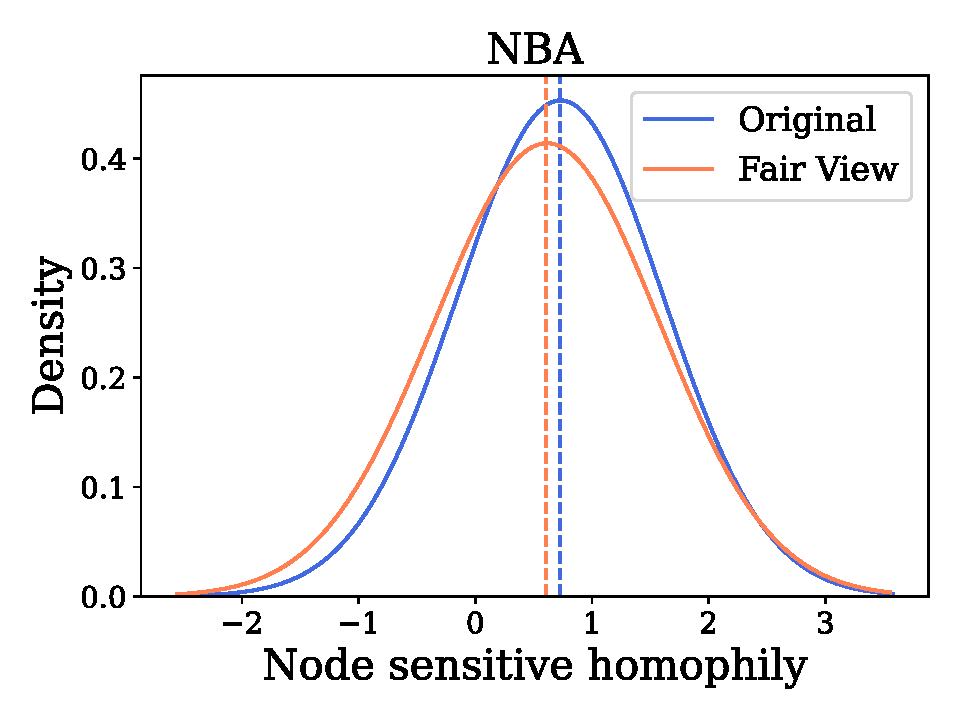
\includegraphics[width=0.32\textwidth]{images/graphair_NBA_nsh.pdf}
    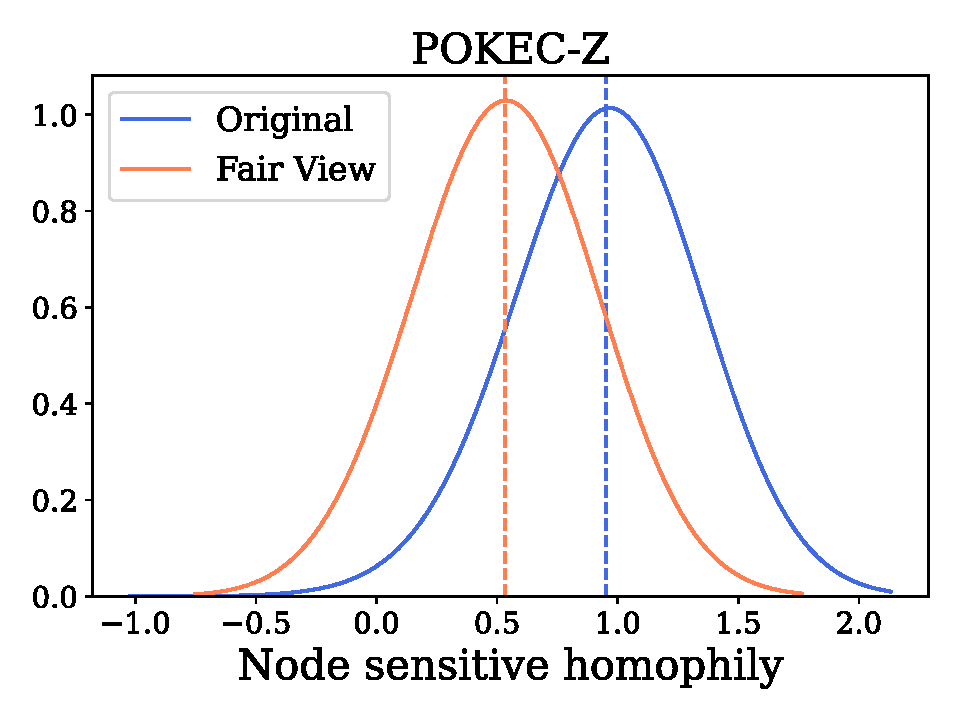
\includegraphics[width=0.32\textwidth]{images/graphair_POKEC_Z_nsh.pdf}
    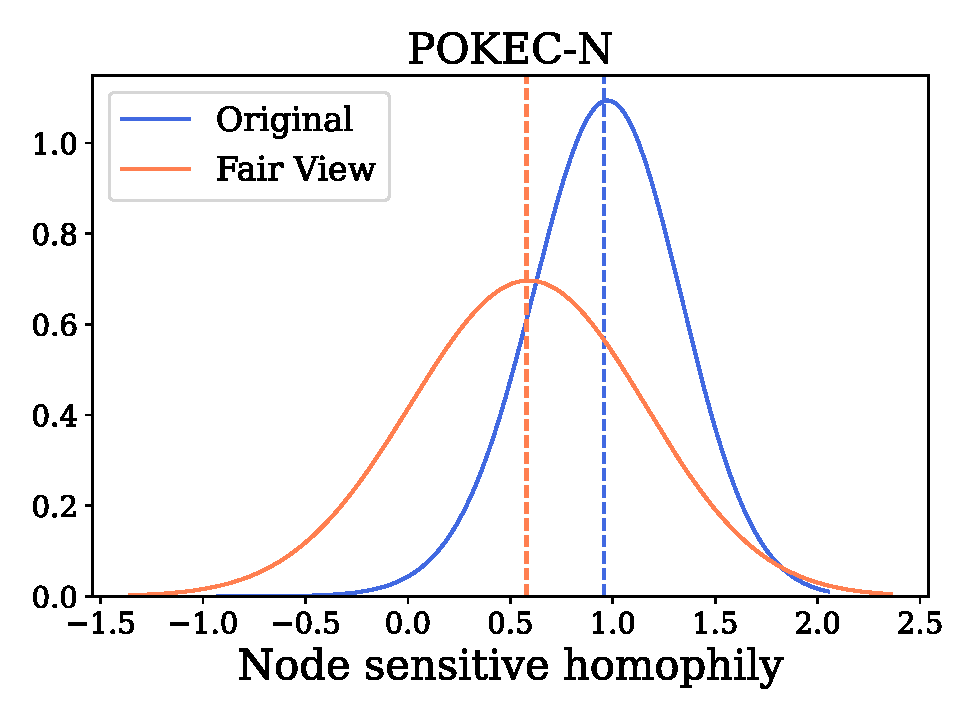
\includegraphics[width=0.32\textwidth]{images/graphair_POKEC_N_nsh.pdf}
    \caption{Distributions of node-wise sensitive homophily in the original and the fair graph data.}
    \label{fig:node-sensitive_homophily}
\end{figure}

\begin{figure}[t]
    \centering
    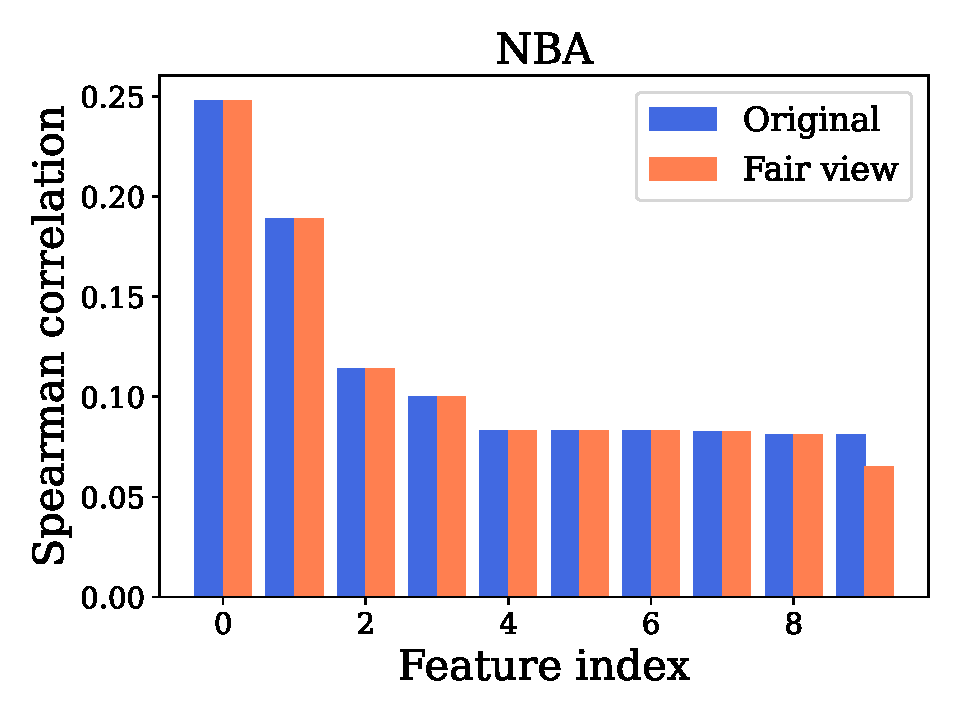
\includegraphics[width=0.32\textwidth]{images/graphair_NBA_correlation.pdf}
    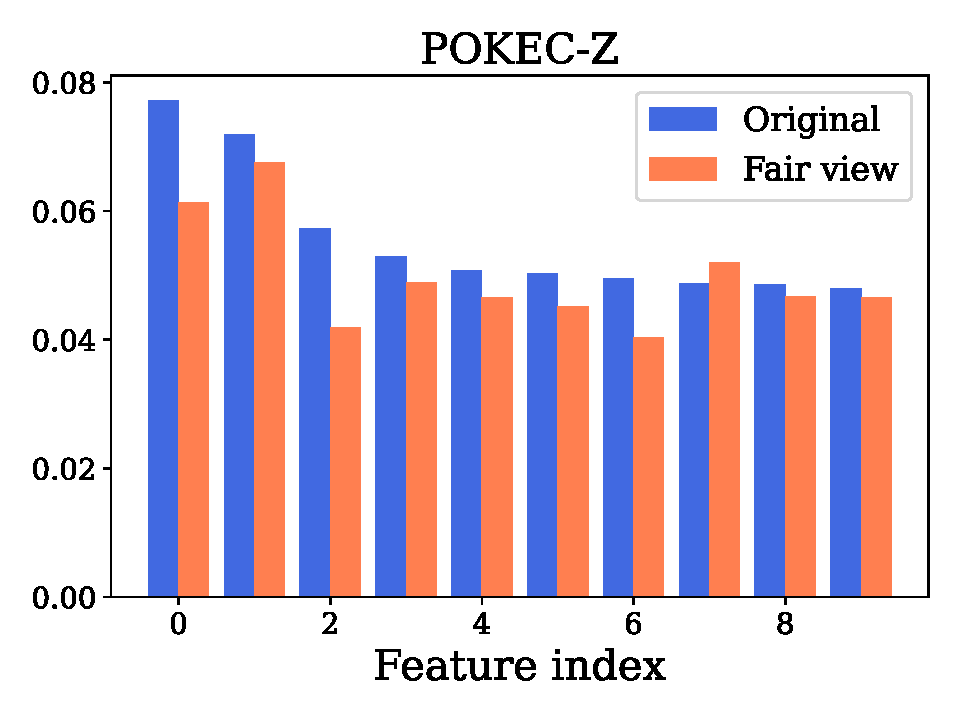
\includegraphics[width=0.32\textwidth]{images/graphair_POKEC_Z_correlation.pdf}
    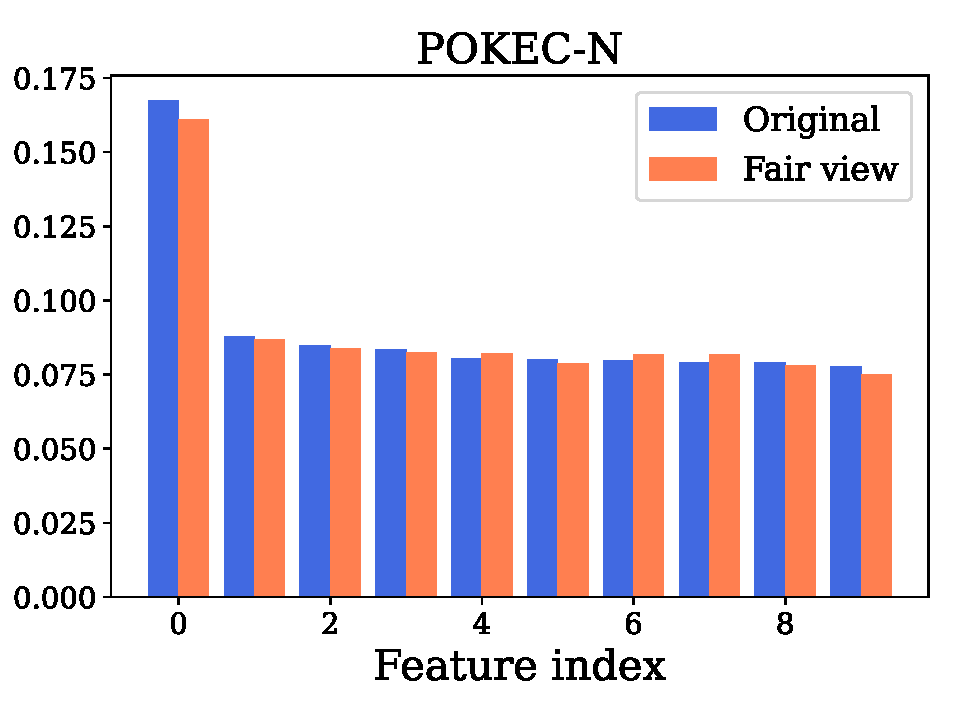
\includegraphics[width=0.32\textwidth]{images/graphair_POKEC_N_correlation.pdf}
    \caption{Spearman correlation between the sensitive feature and the other node features in the original and the fair graph data.}
    \label{fig:correlation}
\end{figure}
